%%insert blank page
%\newpage\null\pagestyle{plain}\newpage
%
%% header with section title
%\pagestyle{fancy}
%\fancyhf{}
%\renewcommand{\sectionmark}[1]{\markright{#1}} %no number
%\fancyhead[le,ro]{\nouppercase{\rightmark}}
%\fancyfoot[le,ro]{\thepage}
%\renewcommand{\headrulewidth}{.4pt}
%\renewcommand{\footrulewidth}{.4pt}

%!TEX root = ../dissertation.tex
\begin{savequote}[75mm]
»Wir sehen in der Natur nie etwas als Einzelheit, sondern wir sehen alles in Verbindung mit etwas anderem, das vor ihm, neben ihm, hinter ihm, unter ihm und über ihm sich befindet.«
\qauthor{Johann Wolfgang von Goethe}
\end{savequote}

\chapter[miRNeo: Creation of a Comprehensive Connectomics Database]{miRNeo: Creation of a\\Comprehensive Connectomics Database} \label{sec:database}
Natural philosophy, as represented by the thought of Johann Wolfgang von Goethe, wants to holistically describe nature and explain and interpret its particular mechanisms. Although natural philosophy is the predecessor of modern, empirical science, its concepts and approaches are still valuable in today's data driven world. As the data we collect grows to dimensions that can only be interpreted with the aid of computers, functional reductionism becomes a valuable paradigm: By studying the facets of nature, we strive to understand it as a whole. Similarly, we regularly encounter Goethe's paraphrase of »all things are connected« in neuro-immunology and in transcriptional connectomics.

\newthought{Bioinformatic support in connectomics} is indispensable, which can be seen by the sheer multitude of possible interactions between the participating factors. However, when I began working on this project (October 2015), there was no integrative database available for this purpose. Earlier that year, miRWalk 2.0 had been published, for the first time providing a relatively comprehensive source of predicted as well as experimentally validated \ac{mir} targeting data\cite{Dweep2015} (see \ref{sec:intro:mirna}). One year later, Marbach's »regulatory circuits« were published,\cite{Marbach2016} enabling analysis of comprehensive \ac{tf}$\to$gene relationships in 394 human tissues (see Section \ref{sec:intro:tf}). These collections (as well as the data they were derived from) are the basis of the database further called \textit{miRNeo}, the development of which will be described in the following chapter.

Since a large part of the scientific progress of this dissertation deals with practical problems of multimodal connectomics, I will begin by describing the infrastructure that makes effective computation of these problems possible. After this technical description of database structure and creation, I will explain the types and organisation of its content. The remainder of the chapter will then deal with the application of this infrastructure to real-world problems in transcriptional connectomics, and the statistical approaches suited to this special case.

%%%%%%%%%%%%%%%%%%%%%%%%%%%%%%%%%%%%%%%%%%%%%%%%
%%%%%%%%%%%%%%%%%%%%% SECTION %%%%%%%%%%%%%%%%%%%%%
%%%%%%%%%%%%%%%%%%%%%%%%%%%%%%%%%%%%%%%%%%%%%%%%

\section{miRNeo - Implementation}
For any biological question to be asked in a bioinformatics setting, the effectiveness of the computational query determines the practicality of the approach. Because resources (i.e., processing power, storage, and working memory) are limited, the database that is queried should be organised in a way that facilitates retrieval of the desired information without excess processing of useless information, for instance, reporting the absence of a connection. In the simplified case of only \acp{mir} interacting with genes in one direction (\ac{mir}$\to$gene), this means retrieval of only those interactions relevant for the queried genes or \acp{mir}. 

Traditional table-based approaches (also known as relational databases) such as \acs{sql}  (»Structured Query Language«) cannot provide such an implementation, since individual entries for genes and \acp{mir} (rows and columns) have to be accessed in their entirety, whether there is a connection between gene and \ac{mir} (1) or not (0). Additionally, adding layers to these interactions (e.g., distinct prediction algorithms, tissues, or the interaction between \acp{tf} and genes) require the addition of entire tables the same size as the database, which is detrimental to effective use of space; and more complex queries also necessitate the transfer of information between those distinct tables (in \ac{sql} typically via a \textcolor{dkblue}{JOIN} command), which claims additional working memory and processing time. Overall, the so-called »many-to-many« organisation of data does not lend itself to representation in a relational database. 

The actual performance is determined by the processing power of the machine it is running on and several structural properties, such as organisation, indexing, monotony, and of course the size of the database; therefore, an estimation of processing time for queries is bound to be inaccurate. However, processing times typically do not vary on the scale of orders of magnitude, and thus general estimations can be made. Well optimised \ac{sql} databases with a size of 5 to 10 GB on disk usually require tens of minutes if not hours to complete one single complex query;\cite{Chaudhuri2004} \textit{miRNeo} in its current form takes up approximately 15 GB of storage. Since one analysis typically consists of several hundreds (and, in the case of permutation analyses, several hundreds of thousands) of these queries, processing times in \ac{sql} implementation are too long to be practically useful. (It seems important to note that, as of 2018, \ac{sql} also offers a graph-based organisation in addition to the traditional, relational layout. These two are separate systems, and not to be confused. The advantages of Neo4j as explained in the following should be seen from the perspective of 2015, when the database was established, and when there was no graph-based \ac{sql} implementation.)

\subsection{Neo4j: A Graph-Based Infrastructure}
To query and display biological data that are organised in a network-like structure (many-to-many), a database that lends itself to the efficient processing and storage of network data is optimal. »Neo4j« utilises a database structure that is built on the save and recall of data points in \emph{nodes} and \emph{edges}, which represent entities (nodes) and relationships between those entities (edges); both nodes and edges can have any number of attributes and a unique property called »type«, usually describing the class of the entry (such as \emph{gene} or \emph{miRNA}). This database organisation replicates the network-like structure of the biological data studied (Fig.\,\ref{fig:graph-org}). Neo4j combines this network-like data structure with an efficient indexing system for quickly finding the entries queried for, and then »walks« along the edges of the nodes that have been found, thus only searching and returning the data that is relevant to the current query. Theoretically, this makes the database more likely to be efficient in the setting of transcriptional interactions, an estimation that turned out to be true.

\begin{figure}
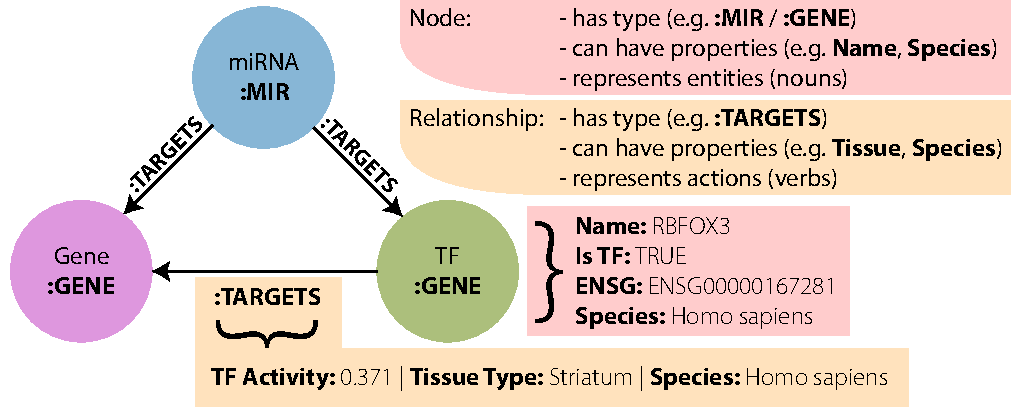
\includegraphics[width=\textwidth]{figures/graph-org}
\caption[Organisation of a Graph Database.]{\textbf{Organisation of a Graph Database.} A graph consists of two basic building blocks: \textit{Nodes}, representing entities, and \textit{edges}, representing connections between entities. Each database entry (node or edge) is an instance of a particular \textit{type} and can possess an arbitrary amount of \textit{properties} detailing its specifics.
\label{fig:graph-org}}
\end{figure}

Depending on the input, these queries can also be rather large; however, the main pitfall of tabular databases such as \ac{sql} is circumvented: there is no need to process entire rows or columns of the table to make sure that the query is satisfied in its entirety. This is particularly useful in a setting of sparse information. To illustrate: only 30 of the 2588 \acp{mir} target a specific gene, which is common; a relational database, after finding the index of the queried gene, would have to search 2588 fields for $1/0$. The graph database, on the other hand, has to execute only 30 searches (or, more accurately, 30 »walks« along the edges connected to the indexed node). In practice, even in the very first prototype implementations, this accelerated standard-case computations immensely, and was even able to accommodate advanced approaches in situations that had been inaccessible in the tabular implementation.

\subsection{High-throughput Database Generation}
Neo4j provides several \acs{api} (»application programming interface«) possibilities in implementation. For the purpose of entering large amounts of data into the database at once, the Java implementation is superior to the other forms in that it provides a batch processing mode via its \texttt{BatchInserter} class. I thus wrote a custom Java program for the purpose of creating an initial state of the database from the largest set of data, the complete miRWalk 2.0 content with 12 algorithms and validated interactions. The downloaded data was organised in a plain text based file format, with one text file for each \ac{mir}, totalling in size about 6 GB (for \textit{H. sapiens}). The database was set up in a way that allows only one node for each individual \ac{mir} and gene entered to avoid duplications, using the commands 
\begin{itemize}[noitemsep, leftmargin=.5cm, label={\tiny\raisebox{.5ex}{\textbullet}}]
\item \texttt{createDeferredConstraint()}
\item \texttt{assertPropertyIsUnique()}
\item \texttt{createDeferredSchemaIndex()} 
\end{itemize}
of the Neo4j Java package. This approach made sure to create only one node for each \ac{mir} (type: MIR) and gene (type: GENE) in the data, which is essential for proper functioning of the database. Each of these nodes received several properties to store individual data, such as the various gene/\ac{mir} identifiers, miRNA sequence, and species. 

Between those basic nodes, the batch insertion process created edges for each relationship that was found in the original data, assigning a type identifier to each edge detailing the origin of this interaction (type: name of the prediction algorithm or »VALIDATED« for experimental data). Thus, while the nodes for genes and \acp{mir} themselves are unique, an arbitrary number of relationships can exist between any two nodes, depending on how many interactions they share.

\subsection{Maintenance and Quality Control}
All additional datasets, such as the \ac{tf} regulatory circuits or \ac{trf} targeting predictions, were entered into \textit{miRNeo} using the regular operation mode. Testing was also performed in regular operation, with manual as well as automated tests to assert the correct transfer of information from raw data to the graph database, and to avoid unpredictable behaviour. At times, conflicts had to be resolved manually, for instance when \ac{mir} names conflicted between old »\ac{mir}*« and new »3p/5p« notation; all manual edits are documented in the code, which was published alongside Lobentanzer \emph{et al}.\cite{Lobentanzer2019a}

Except for the rapid import of large amounts of data in creation of a database, the Java implementation of Neo4j does not offer many advantages over the native R implementation, »RNeo4j«. Thus, after creation and a short period of experimentation with graphical user interfaces, I abandoned the Java program in favour of the more flexible R programming. While Java is an object-based programming language, whose benefits lie in extreme flexibility in regards to platform and purpose, high modularity, and speedy processing, R as a procedural language is the work horse of modern bioinformatics. Its procedural design (the division of data and functions that operate on that data) facilitates the transfer of approaches between distinct datasets, and the enormous vibrant community of data scientists using R provides a wealth of third party packages to tackle almost any bioinformatic task. In the remainder of this dissertation, all analyses are performed in R, unless specifically stated otherwise.

%%%%%%%%%%%%%%%%%%%%%%%%%%%%%%%%%%%%%%%%%%%%%%%%
%%%%%%%%%%%%%%%%%%%%% SECTION %%%%%%%%%%%%%%%%%%%%%
%%%%%%%%%%%%%%%%%%%%%%%%%%%%%%%%%%%%%%%%%%%%%%%%

\section{miRNeo - Materials}
All materials used in the creation of \textit{miRNeo} have been acquired from resources that are non\-/commercial, web-available, and open-source (in the case of code). All properties and relationships derived from this data were entered into \textit{miRNeo} as either nodes, properties of nodes, edges, or properties of edges. 

\subsection{Gene Annotation}
Even though »regular« protein coding genes have been known for a long time, there is no consensus yet about their nomenclature and organisation. Complicated by newly discovered functions and properties of phylogenetic nature, the scientific representation of the human genome is in constant flux. Several large organisations strive to provide a robust annotation of the human gene catalog, but also in many cases contradict one another. There are three nomenclature systems that are of high importance in modern genomics: 
\begin{itemize}[noitemsep, leftmargin=.5cm, label={\tiny\raisebox{.5ex}{\textbullet}}]
\item The traditional naming system of acronyms (e.g. \ac{chat}) and fantasy-names (such as »Sonic Hedgehog«), also occasionally called »gene symbol«, is still widely popular because of its accessibility to humans, but is also not particularly robust because of a high amount of synonyms with high confusion potential (see e.g. Section \ref{sec:intro:neurokine} on CDF) and instances of genes without names having to carry unwieldy systematic names. Gene symbols are largely, but not exclusively, curated by the HUGO Genome Nomenclature Consortium (HGNC), under the roof of the Human Genome Organisation (HUGO). As such, there also exists an »official« HGNC symbol for many genes, but these are not consistently used throughout the literature.
\item The American \ac{ncbi}, a branch of the National Institute of Health (NIH), curates and hosts a multitude of biological and medical data, and for the organisation of gene information uses its own systematic nomenclature termed »Entrez« ID. Entrez is a molecular biology database that integrates many aspects of biology and medicine in a gene-centred manner, and therefore Entrez IDs are useful to quickly connect a gene to its function, nucleotide sequence, or associated diseases. Entrez IDs are regular integers without additional characters.
\item Akin to the \ac{ncbi} effort, ENSEMBL is a project of the European Bioinformatics Institute (EBI) as part of the European Molecular Biology Laboratory (EMBL). Compared to the Entrez database, it is more focused on study and maintenance of the genome itself, and therefore has a more intricate nomenclature that allows for differentiation of, for example, genes and their various transcript isoforms (ENSEMBL IDs carry character prefixes for class identification, e.g., ENSG for genes, ENST for transcripts).
\end{itemize}
All of these are being used on a regular basis in many publications, and, often, they are used exclusively. As a result, the end user of the published data has to have access to all possible annotation forms, or, at least, a means to translate one into the other; often, this also introduces conflicts. For this reason, all ID types were entered into \textit{miRNeo} upon creation or during maintenance, for convenience and to minimise analysis prolongations due to conflict resolution.

\subsection{microRNA Annotation}
miRBase provides a consistent annotation for \acp{mir}. Due to their relatively recent discovery, there still are major changes from version to version; the syntax, however, is stable. In addition to the \ac{mir} »names« that are composed of species, the string »miR«, pre-\ac{mir} designation number, and strand origin (e.g. »hsa-miR-125b-5p«), miRBase provides IDs for pre-\ac{mir} molecules (also called ancestors) termed »MIID« and IDs for mature \ac{mir} molecules termed »MIMAT«. However, in practice, these are rarely used. Similarly, \ac{mir} families are annotated using the »MIPF« ID.

\subsection{Transcription Factor Targeting} \label{sec:database:tf}
The FANTOM5 project has applied \ac{cage} to a large number of human samples from diverse tissues to determine the accurate 5' ends of each transcript.\cite{Hon2017} Knowledge of this fact enables accurate prediction of transcription factor binding sites likely to control a transcript's expression. Marbach and colleagues used this information in combination with detailed human gene expression data to derive a complex interaction network of \acp{tf} and genes (»regulatory circuits«), and in doing so aggregated samples with similar expression patterns and origins into 394 fictional tissues.\cite{Marbach2016} For every tissue, each \ac{tf} was assigned transcriptional activities towards all genes that it supposedly targets (with the sum of all activities in any given tissue being \num{1}). Marbach and colleagues have shown that the cumulative transcriptional activities towards any given gene correlate well with the actual gene expression in corresponding samples from an independent repository.

Even in its fifth iteration, FANTOM data is not entirely comprehensive, which came to my attention due to a cholinergic anomaly: The 5' \ac{cage} peaks of the \textit{\ac{chat}} and \textit{\acs{a7}} (the nicotinic $\alpha$7 receptor subunit) genes in raw FANTOM5 brain tissue data do not pass the expression threshold, and therefore are not included in, e.g., Marbach's »regulatory circuits«. Both are critically important not only for neuronal cholinergic systems, but also for the non-neuronal aspect of immune processes. For instance, macrophages have been shown to produce \ac{ach} via \ac{chatp}, and the $\alpha$7 homomeric \ac{ach} receptor conveys direct immune suppression by its expression on monocytes.\cite{Fujii2017} Paradoxically, the \ac{cage} peak of \textit{\ac{slc}}, which lies in the first intron of \textit{\ac{chat}}, crosses the threshold and therefore is included in the data. Unfortunately, I was not able to remedy these circumstances even upon personal communication with Daniel Marbach (author of »regulatory circuits«) and Hideya Kawaji of the FANTOM5 consortium, although the latter acknowledged the possibility of a gene annotation deficit leading to misattribution of the \textit{\ac{chat}} signal to \textit{\ac{slc}} due to the closeness of their 5' ends. Thus, it seems viable to substitute \emph{SLC18A3} targeting data for the absent \emph{CHAT} data in certain situations.

The entire collection of transcriptional activities in all tissues was downloaded from the project's web page,\cite{Marbach2016} and neuronal and immune tissues were manually curated and entered into \textit{miRNeo}. The collected data comprises 33 neuronal tissues and 26 immune cell tissues (Appendix \ref{appendix:marbach}), and \num{1130196} \ac{tf}$\to$gene relationships in total (not all 394 tissues were entered due to the time requirements). 

\subsection{microRNA Interactions} \label{sec:database:mirna}
The content of miRWalk 2.0 is freely available online;\cite{miRWalk2} however, there is no option of downloading the complete set. The targeting data thus was downloaded per \ac{mir} using a custom crawler, with standard options for all 12 prediction algorithms (miRWalk, miRDB, PITA, MicroT4, miRMap, RNA22, miRanda, miRNAMap, RNAhybrid, miRBridge, PICTAR2, and TargetScan) in plain text format. For experimentally validated interactions, the main sources were DIANA TarBase\cite{Karagkouni2018} and miRTarBase,\cite{Chou2018} both of which offer complete download options. As of 2019, the 3.0 version of miRWalk allows complete species downloads; however, the developers have abandoned their third party algorithm plurality reducing the number of available alternatives from 12 to 4, which can be considered a significant disadvantage, as is described in the next paragraph.

While sequence complementarity, particularly of the »seed«-region, is the primary paradigm of \ac{mir}-mRNA interaction, prediction algorithms vary widely in their implementation, general purpose, and approach to interaction prediction (for a comprehensive review of approaches and rules, see Yue \emph{et al.}\cite{Yue2009}). A large group of available options utilise sequence conservation aspects to increase candidate viability (such as miRanda, PicTar, TargetScan, and microT4). Others, such as RNA22 and PITA, utilise biophysical aspects such as free energy of binding or the accessibility of target sites due to secondary RNA structures as prediction arguments. All of these approaches have their up- and downsides, e.g. considering their general precision and sensitivity, or their adequate prediction of particular cases, such as multiple site targeting. Thus, it has been proposed to use a combination of complementary approaches instead of only one algorithm per analysis.\cite{Witkos2011} For this reason, I may have preferred the 2.0 version of miRWalk, even if 3.0 had been available at the time.

One advantage of the collection of all data in a quickly accessible database is the opportunity to compare the different approaches to target prediction. A statistical evaluation of the collected interaction data from miRWalk 2.0 showed vast differences in general prediction quantity (Table \ref{tab:alg.hit.freq.all}) as well as prediction accuracy and sensitivity when compared to the validated subset of data (Table \ref{tab:alg.hit.freq.val}). Since the ground truth is not known, this is an additional argument for the combination of multiple algorithms instead of the use of a single set. Apart from RNAhybrid and miRBridge, all algorithms presented reasonable base hit frequencies and increases in the validated test set. While miRBridge already has the lowest positive frequency of all the algorithms, it is the only one to achieve a negative score in the validated test set. On the other hand, RNAhybrid has a vastly higher base hit frequency than the second highest scoring algorithm (by more than \num{300}\%), making it very likely to produce false positive results, and less valuable in the aggregation scoring system. The remaining ten algorithms were included in \textit{miRNeo} targeting data. For ease of use, an additional relationship type was created from the aggregated single algorithm hits of any \ac{mir}$\to$gene relationship, with the sum of algorithms predicting the interaction as a score variable. This yields a theoretical score range from \num{3} to \num{10} (\ac{mir}$\to$gene relationships with only one or two hits were ignored for the sake of space). To account for experimentally validated interactions, each \ac{mir}$\to$gene relationship that was supported by strong evidence of interaction was modified by addition of \num{10.5} score points (a half point for quick identification of a validated relationship), extending the maximum score to \num{20.5} points. The resulting optimised graph contains \num{11687931} human \ac{mir}$\to$gene targeting relationships with a distinct score distribution (Fig.\,\ref{fig:db-score-hist}). In comparison, only 6146 \ac{mir}$\to$gene relationships are experimentally validated with »strong« evidence.

\begin{figure}
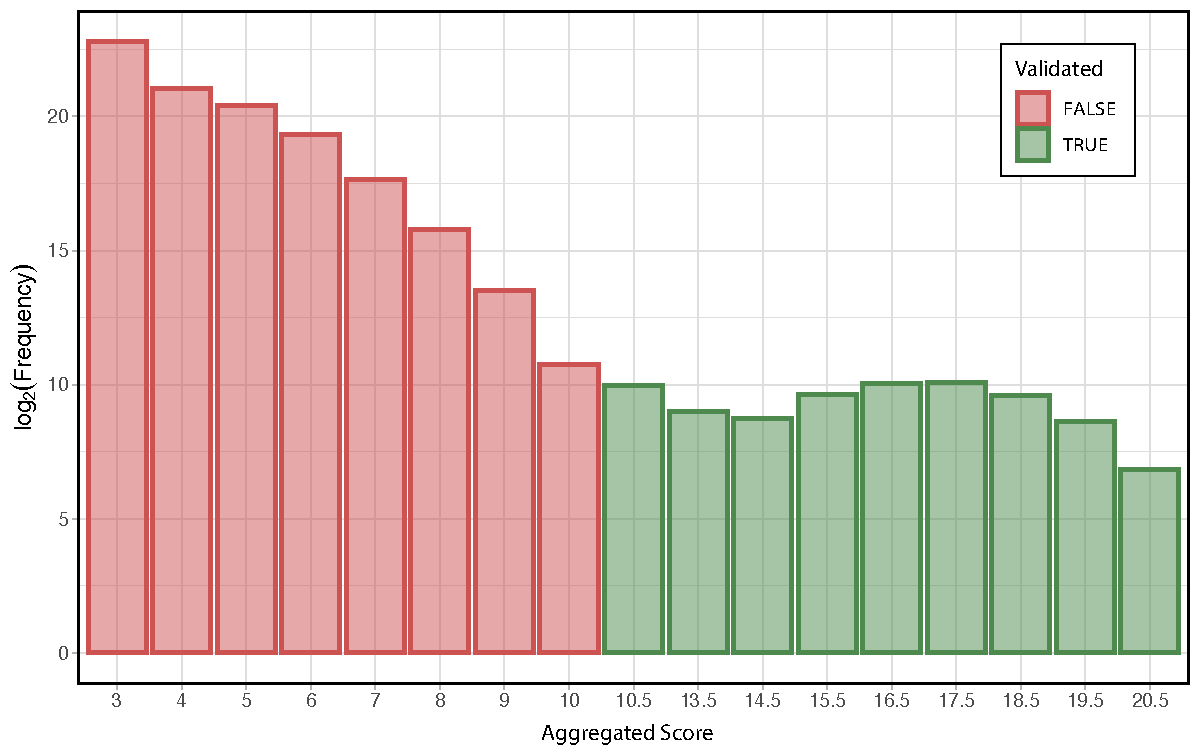
\includegraphics[width=\textwidth]{figures/db-score-hist}
\caption[Histogram of \ac{mir}$\to$Gene Score Distribution.]{\textbf{Histogram of \ac{mir}$\to$Gene Score Distribution.} Aggregation of individual algorithms yields a score range of 3 to 10 per individual \ac{mir}$\to$gene interaction. In case of additional existence of experimental validation (evidence level high) for any predicted interaction, score is increased by 10.5. The distribution shows a sharp decrease in predicted interactions towards higher scores, and a maximum of validated interactions at prediction scores 6 and 7. 
\label{fig:db-score-hist}}
\end{figure}

%tables from cholinomir pseudopaper
\begin{table}
\sffamily
\small
%\resizebox{.85\textwidth}{!}{%
\noindent\parbox[t]{.35\linewidth}{
\centering
\begin{tabular}{c | c}
algorithm & hit frequency\\ \hline
\hline
\textcolor{Maroon}{RNAHYBRID} & 71.62\%\\ \hline
\textcolor{OliveGreen}{MIRMAP} & 19.90\%\\ \hline
\textcolor{OliveGreen}{MIRWALK} & 19.74\%\\ \hline
\textcolor{OliveGreen}{TARGETSCAN} & 16.33\%\\ \hline
\textcolor{OliveGreen}{RNA22} & 12.34\%\\ \hline
\textcolor{OliveGreen}{MICROT4} & 11.81\%\\ \hline
\textcolor{OliveGreen}{MIRANDA} & 10.65\%\\ \hline
\textcolor{OliveGreen}{PITA} & 4.90\%\\ \hline
\textcolor{OliveGreen}{MIRDB} & 1.17\%\\ \hline
\textcolor{OliveGreen}{MIRNAMAP} & 0.75\%\\ \hline
\textcolor{OliveGreen}{PICTAR2} & 0.62\%\\ \hline
\textcolor{Maroon}{MIRBRIDGE} & 0.15\%\\ \hline
\end{tabular}
\caption{Prediction algorithms ordered by the fraction of all possible interactions they predict as being real (positive rate). Different algorithms display a wide variation of hit rates in the entirety of predicted interactions between any \ac{mir} and gene. Red: excluded from analysis.}
\label{tab:alg.hit.freq.all}
}
\hfill
\noindent\parbox[t]{.6\linewidth}{
\begin{tabular}{c | c | c}
algorithm & validated hit frequency & hit rate increase\\ \hline
\hline
\textcolor{OliveGreen}{PICTAR2} & 6.98\% & 1129.40\%\\ \hline
\textcolor{OliveGreen}{MIRDB} & 9.80\% & 838.43\%\\ \hline
\textcolor{OliveGreen}{MIRANDA} & 51.73\% & 485.94\%\\ \hline
\textcolor{OliveGreen}{TARGETSCAN} & 70.63\% & 432.51\%\\ \hline
\textcolor{OliveGreen}{MIRNAMAP} & 3.10\% & 410.95\%\\ \hline
\textcolor{OliveGreen}{PITA} & 15.57\% & 317.20\%\\ \hline
\textcolor{OliveGreen}{MICROT4} & 32.60\% & 276.10\%\\ \hline
\textcolor{OliveGreen}{MIRMAP} & 53.86\% & 270.65\%\\ \hline
\textcolor{OliveGreen}{MIRWALK} & 50.95\% & 258.15\%\\ \hline
\textcolor{OliveGreen}{RNA22} & 22.51\% & 182.38\%\\ \hline
\textcolor{Maroon}{RNAHYBRID} & 90.47\% & 126.32\%\\ \hline
\textcolor{Maroon}{MIRBRIDGE} & 0.01\% & 0.00\%\\ \hline
\end{tabular}
\caption{Prediction algorithms ordered by their increase in true positive rate when considering only validated interactions. The hit rate increase when comparing experimentally validated interactions with the entire predicted data (Table \ref{tab:alg.hit.freq.all}) is also subject to strong variation. Hit rate increase is the increase of hit rate if only considering validated data as opposed to all predicted interactions. None of the studied algorithms unite a good precision (hit rate increase) and coverage (validated hit frequency).}
\label{tab:alg.hit.freq.val}
%}
}
\end{table}

\subsection{Filtering of Aggregated Prediction Scores}
For the estimation of the »true« \ac{mir}$\to$gene interactions in the predicted-only data in \textit{miRNeo}, two premises are relevant: First, the enormous amount of hits with a score of 3 in all likelihood is an over-estimation, and second, the amount of currently validated interactions can be but a small fraction of »true« interactions. Assuming the truth lies on the axis between these two extremes (i.e., at some score value inside the \textit{miRNeo} interactions), the true amount of human \ac{mir}$\to$gene interactions must approximately fall within the range of $2^{10}$ to $2^{20}$. Looking at the score distribution of all \textit{miRNeo} interactions (Fig.\,\ref{fig:db-score-hist}), the maximum amount of validated interactions is predicted by a combination of six or seven algorithms (i.e., a score of 16.5 or 17.5). Thus, to approximate the true state, I chose to apply a low-cut filter to \textit{miRNeo} queries at a minimum score of 6. This is the standard case referred to as »\textit{miRNeo} query« in the remainder of this dissertation. In some cases, such as the graphical analysis of whole-genome \ac{mir} targeting (see e.g. Section \ref{sec:cellculture:network}), the score threshold was raised to 7 to circumvent computational limitations.

\subsection{De-novo Prediction of tRF Targeting} \label{sec:database:trf-targeting}
Due to the recency of their (re-)discovery, no comprehensive interaction sources exist for \acfp{trf}. There have been documented cases of \ac{mir}-like behaviours of distinct RNA fragments,\cite{Cole2009,Kumar2014} justifying an attempt to predict interactions in a comprehensive manner. Of the available options for nucleotide interaction prediction algorithms, TargetScan\cite{Friedman2009} seems particularly suited for this task because it provides the option of evaluating the evolutionary conservation of target sites in the putatively targeted genes, thereby providing an additional layer of security: The sequence of 3' \acp{utr} is evolutionarily less stable than the coding part of genes; thus, high conservation of the binding site may indicate evolutionary pressure to keep up the interaction with the fragment, making an actual function of the interaction more likely. TargetScan also presents with reasonable sensitivity and specificity as confirmed by an independent group,\cite{Alexiou2009} and through an additional algorithm allows the attribution of a score based on the branch length (on the species tree) of conserved targeting.\cite{Agarwal2015}

\ac{mir}-like behaviour implies the existence of a region on the \ac{trf} similar to a \ac{mir} »seed«, and TargetScan also expects a seed as input to its targeting algorithm. Since there has been no definitive answer to the question as to where the seed region in \acp{trf} may be, it is safest to assume nothing and explore all possibilities, i.e., simulate every possible seed position for interaction discovery. For this purpose, all discovered sequences of \acp{trf} (exceeding a base mean expression of 10 counts) were chopped into 7-nt pieces (7mers), which is the length of \ac{mir} seeds, and statistically improbable enough to appear in the genome at random; the average length of a human 3' \ac{utr} is 800 \ac{nt}, so the probability of finding any 7mer randomly in any one 3' \ac{utr} is $p = \frac{800}{4^7} = 0.049$, which agrees with the 5\% \ac{fdr} convention.

\subsection{microRNA Primate Specificity}
During the course of evolution, higher organisms typically attained more complexity in a variety of functional categories. The \ac{cns} as the system of highest complexity underwent several drastic developments from invertebrates to lower mammals to higher mammals still. miRNAs are no exception. While many miRNAs are functionally as well as literally conserved in all mammals, primates in particular have gained a substantial amount of novel miRNAs whose function is in large parts elusive. Due to the restrictions on experimentation on higher mammals, particularly primates, many of those miRNAs can only be studied observationally, or by transgenic experiments in rodents. A cholinergic example of a gain-of-function in higher mammalian miRNA regulation is the vesicular acetylcholine transporter, \ac{slc}. As described in Section \ref{sec:database:tf}, the \ac{slc} gene is situated in the first intron of \ac{chat}, and thus is always primarily co-expressed with the latter. However, a primate-specific miRNA, miR-298, targets the 3' UTR of \ac{slc}.\cite{Soreq2015} Thus, the primate neuron has gained a mechanism of independent \ac{slc}/\ac{chat} regulation that the mouse, for example, does not possess. It is easily imagined that such a gain of neuronal flexibility, in many instances, can aid the development of a more effective brain. However, the primate specificity of miRNAs is not yet consensus, and thus not found in annotation databases such as miRBase, even though they list all miRNAs discovered in any species. To get an impression of the amount of possible gain of function, I performed a review of miRNAs expressed in a representative variety of annotated species. From hereon out, largely method-related paragraphs will be set in sans-serif font face.

\begin{method}

\subsubsection{Species Selection}
The tested species were selected from miRBase v21. Some of the available species are severely limited in the extent of miRNA annotation, likely because of a research bias. Therefore, only the most well-annotated species were selected. These are (number of annotated primary and mature miRNAs in brackets):
\begin{itemize}[noitemsep, leftmargin=.5cm, label={\tiny\raisebox{.5ex}{\textbullet}}]
\item \emph{Homo sapiens} (human; 1881, 2588)
\item \emph{Gorilla gorilla} (gorilla; 352, 357)
\item \emph{Pan troglodytes} (chimp; 655, 587)
\item \emph{Pongo pygmaeus} (orangutan; 642, 660)
\item \emph{Macaca mulatta} (rhesus macaque; 619, 914)
\item \emph{Bos taurus} (cow; 808, 793)
\item \emph{Canis familiaris} (dog; 502, 435)
\item \emph{Mus musculus} (mouse; 1193, 1915)
\item \emph{Rattus norvegicus} (rat; 495, 765)
\end{itemize}
The first four species belong to the hominid group; the first five are primates. It is likely that these collections are not complete, with the degree of completeness depending on the amount of research performed on the species (as demonstrated, e.g., by the difference between mouse and the other non-primates). This places considerable difficulty on asserting primate specificity of miRNA, and in turn on assertion of the effects of evolution on the miRNA regulatory system.

\subsubsection{Single miRNA Inter-Species Homology Computation}
To determine the homology of miRNAs between the studied species, reference genomes were downloaded from the respective sources and analysed phylogenetically, using the genomic coordinates provided by miRBase. Homology of sequences was determined via dynamic programming using the Smith-Waterman algorithm.\cite{Smith1981} Briefly, this algorithm can be used to determine the similarity of two genomic sequences, based on a scoring system rewarding matches and penalising mismatches. Smith and Waterman extended the original approach by Needleman and Wunsch,\cite{Needleman1970} which is used to compare two complete sequences. Both algorithms rate an alignment by dynamic scoring inside a 2D-matrix, with the sequences to be compared as the x- and y-axes (one letter per cell). By a change in the scoring system, the Smith-Waterman algorithm finds the best local alignments, instead of comparing the two sequences in their entirety. In the case of miRNAs, this behaviour is useful because, between species, there are frequent additions or deletions of single \ac{nt} on both ends of the homologous miRNA. Genomes were procured from the following sources:
\begin{itemize}[noitemsep, leftmargin=.5cm, label={\tiny\raisebox{.5ex}{\textbullet}}]
\item \emph{Homo sapiens}: GRCh38 (NCBI)
\item \emph{Gorilla gorilla}: gorGor3 (UCSC)
\item \emph{Pan troglodytes}: panTro4 (UCSC)
\item \emph{Pongo pygmaeus}: PPYG2 (Ensembl)
\item \emph{Macaca mulatta}: rheMac3 (UCSC)
\item \emph{Bos taurus}: bosTau6 (UCSC)
\item \emph{Canis familiaris}: canFam3 (UCSC)
\item \emph{Mus musculus}: mm10 (UCSC)
\item \emph{Rattus norvegicus}: rn5 (UCSC)
\end{itemize}

Using the genome coordinates provided by miRBase, the genomic sequences of miRNAs and pre-miRNAs of each species were determined. Using the Smith-Waterman algorithm, all identified homologs of human miRNAs were subjected to homology scoring, and score results were visualised as a heatmap.

\end{method}

\begin{figure}
\centering
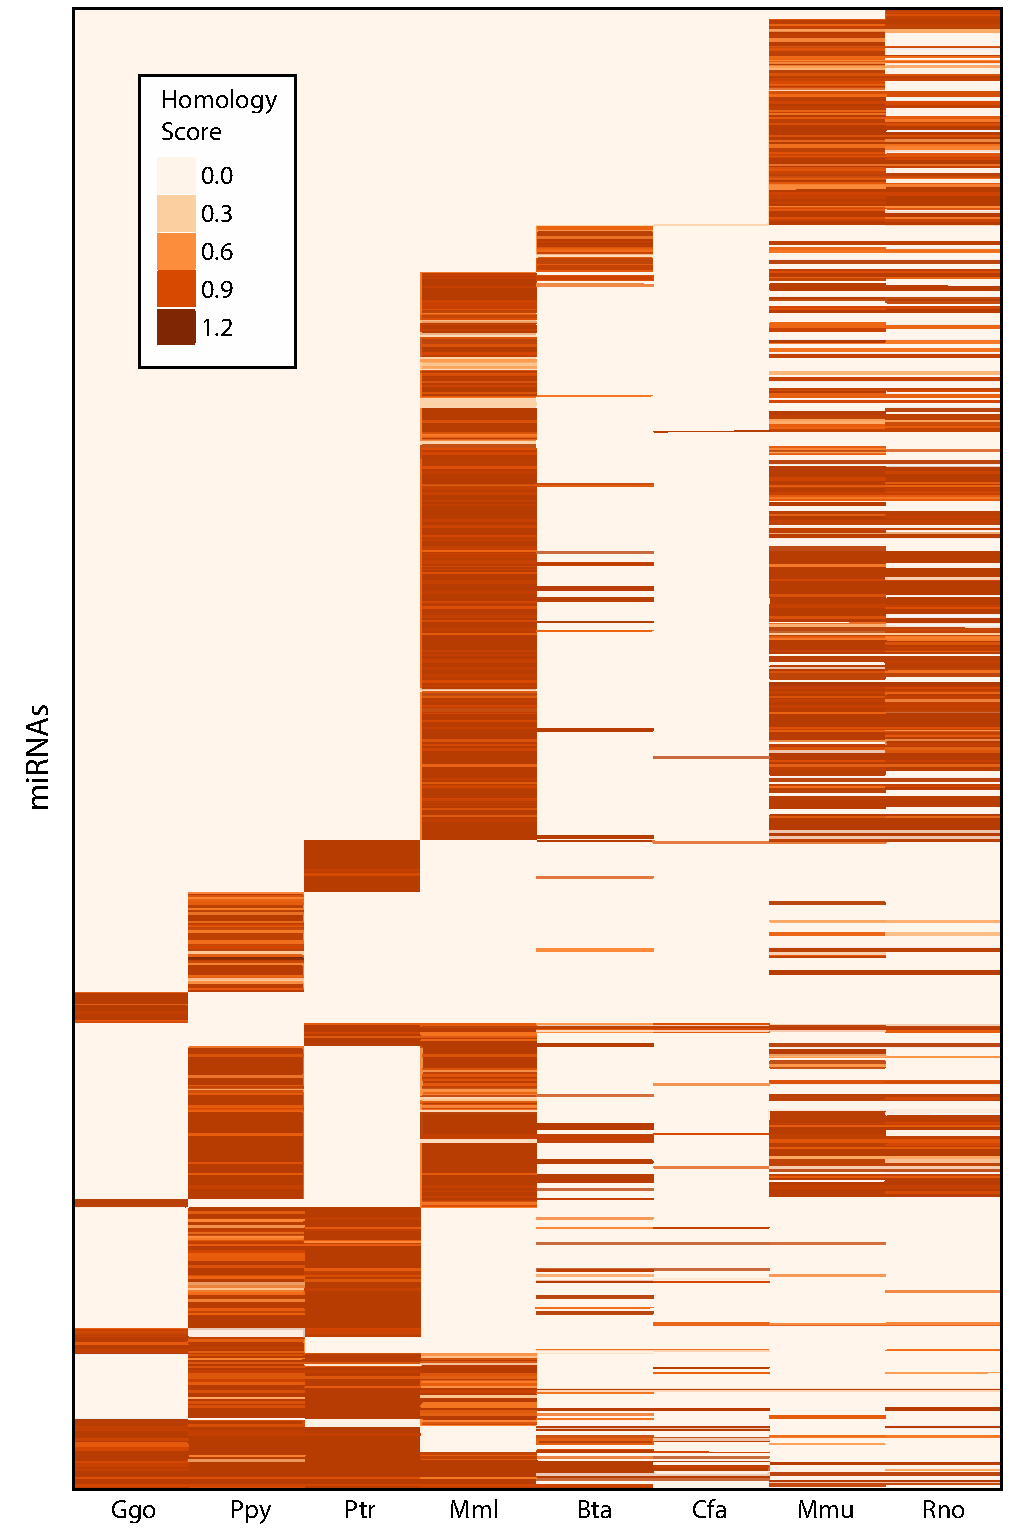
\includegraphics[width=.9\textwidth]{figures/species-homo}
\caption[microRNA Species Homology.]{\textbf{Homologues of Human microRNAs in Primate- and Non-Primate-Species.} Homology to human miRNAs was determined by Smith-Waterman local alignment for each homologous miRNA of 8 species. Homology scores were visualised on a heatmap, each column represents the homology to human of the miRNAs of the respective species. The heatmap is ordered from bottom to top by the amount of miRNA homologues in primates. The miRNAs at the very bottom are shared by human as well as all four primate species, followed by the miRNAs shared by three primate species, and so on. Ggo: \emph{Gorilla gorilla}, Ppy: \emph{Pongo pygmaeus} (Orangutan), Ptr: \emph{Pan troglodytes} (Chimp), Mmt: \emph{Macaca mulatta} (Rhesus macaque), Bta: \emph{Bos taurus} (Cow), Cfa: \emph{Canis familiaris} (Dog), Mmu: \emph{Mus musculus} (Mouse), Rno: \emph{Rattus norvegicus} (Rat).
\label{fig:species-homo}}
\end{figure}

\subsubsection{Inter-Species Distribution of miRNAs}
The inter-species relationships of annotated miRNAs do not follow a simple evolutionary distribution from less complex to more complex organisms, but rather seem to partially result from parallel development (Fig. \ref{fig:species-homo}). Taking into account the high probability of missing annotations in several species (particularly hominids), it seems prudent to define primate specificity of miRNAs not by presence in primates, but rather by absence of the miRNAs in non-primate species (also excluding miRNAs \emph{only} annotated in human). Thus, primate specificity of a human miRNA is assumed if the miRNA is expressed in at least one primate species, and absent from all non-primate species in this roster. This definition yields a list of 377 primary and 350 mature putative “primate specific” miRNAs in miRBase v21 (Appendix \ref{appendix:homologues}). Judging from recent analyses,\cite{Londin2015} there probably exist many more. The primate-specificity attribute was entered into \emph{miRNeo} as miRNA node property.

%%%%%%%%%%%%%%%%%%%%%%%%%%%%%%%%%%%%%%%%%%%%%%%%
%%%%%%%%%%%%%%%%%%%%% SECTION %%%%%%%%%%%%%%%%%%%%%
%%%%%%%%%%%%%%%%%%%%%%%%%%%%%%%%%%%%%%%%%%%%%%%%

\section{miRNeo - Usage} \label{sec:database:usage}
Neo4j uses a language (called »Cypher«) akin to \ac{sql}, which utilises keyphrases to issue commands, but combines it with a semi-graphical syntax to account for the graph-based layout of the data. In the following, I will describe its basic usage and the advantages it provides in the matter of transcriptional connectomics (code examples are simplified for explanatory purposes). The basic »finder« function (similar to \textcolor{dkblue}{SELECT} in \ac{sql}) is called \textcolor{dkblue}{MATCH} in Cypher, and, when combined with the semi-graphical syntax, can be used to identify nodes or more complex patterns in the database. The graphical syntax consists of two main building blocks that represent the basic types of data inside the database: nodes as regular brackets »\textbf{\texttt{( )}}« and edges between nodes as  a construct of hyphens and square brackets, that can also have a direction indicated by the greater sign \mbox{»\textbf{\texttt{( )-\string[ \string]->( )}}«}. To specify the elements to be found, attributes of nodes and/or edges can be filtered by using curly brackets in the node definition, or the \textcolor{dkblue}{WHERE} clause. To be returned, elements need to be assigned arbitrary variable names:

\begin{lstlisting}[label=lst:match, caption=MATCH, language=Cypher]
MATCH (gene:GENE {species: 'HSA'})
WHERE gene.name = 'CHAT'
RETURN gene
\end{lstlisting}

Query \ref{lst:match} identifies a node (arbitrarily designated »gene«) with type GENE (indicated by the colon), with attributes »species« (HSA, i.e. \textit{H. sapiens}) and »name« (\ac{chat}), and returns the node with all its attributes. Since the nodes of type GENE are restrained, there can only be one gene of species \textit{H. sapiens} with this name in the database, and thus, only one data point will be returned. The graphical syntax further allows for pattern matching of, for instance, \ac{mir}$\to$gene relationships:

\begin{lstlisting}[label=lst:pattern, caption=Patterns,
language=Cypher]
MATCH (mir:MIR)-[rel:TARGETS]->(gene:GENE {species: 'HSA'})
WHERE gene.name = 'CHAT'
RETURN mir, rel, gene
\end{lstlisting}

Query \ref{lst:pattern}, similar to query \ref{lst:match}, starts by identifying the node of species HSA with the name \ac{chat}, and proceeds to look for \ac{mir}$\to$gene relationship edges arriving at this node; the relationships have to be of the type TARGETS (the pre-aggregated score-based accumulation of targeting). As soon as no further edges are found, the process terminates and returns all found \acp{mir} (»mir«), relationships (»rel«), and genes (»gene«) in discrete form, including all their attributes, such as the ENSG and Entrez IDs, the MIMAT IDs for all found \acp{mir}, or the score value of their targeting relationship. In this query, since there is a constraint on genes, the only gene returned is \textit{\ac{chat}}. However, Cypher is not limited to filtering on unique attributes; it allows for query and return of as many data points as are needed. For example, if one is interested in all \ac{mir}$\to$gene interactions in the cholinergic system, the query may look as follows:

\begin{lstlisting}[label=lst:filter, caption=Filtering,
language=Cypher]
MATCH (mir:MIR)-[rel:TARGETS]->(gene:GENE {species: 'HSA'})
WHERE gene.name IN {cholinergic_genes}
RETURN mir, rel, gene
\end{lstlisting}

The effectiveness of graph-based databases becomes clear in this approach: Query \ref{lst:filter} is processed starting at a user-defined filter, the list of cholinergic genes as an input (containing \textit{\ac{chat}}, \textit{\ac{slc}}, cholinergic receptor genes, \acl{ache}, etc). In a first step, all nodes are found that fulfil the criteria: type GENE, from species \textit{H. sapiens}, that are in the list of names given. Since the gene nodes are indexed, this only requires milliseconds. Then, through the connection of edges to these nodes, it finds all \ac{mir} nodes that have a \ac{mir}$\to$gene relationship towards any of the cholinergic genes. By using the gene nodes as starting point, the query can end as soon as no other edges fulfilling these criteria are found on any of the nodes. In comparison, to satisfy this query in a relational database, the rows representing these cholinergic genes would have to be assessed in their entirety, not only in those columns that represent an extant relationship, thus prolonging execution.

The database then returns all \ac{mir}$\to$gene relationships in this set, representing the network of cholinergic \ac{mir} regulators, including all of their attributes. The advantages of graph-based data do not end there; say one wants to return only »master« regulators of cholinergic systems, defined as \acp{mir} that target at least 4 of the genes in the cholinergic set. In a relational database, this would have to be done post-hoc, by aggregation of relationships and removal of any results that do not exceed this threshold. This requires storage of the entire result in memory, and additional computational steps that can be very taxing depending on the size of the result table. In Cypher, this can be done during the query (code comments indicated by »\textcolor{dkgreen}{//}« explain single steps):

\pagebreak

\begin{lstlisting}[label=lst:filter2, caption=Two-stage Filtering,
language=Cypher]
MATCH (gene:GENE {species: 'HSA'})
WHERE gene.name IN {cholinergic_genes}
WITH gene //the found genes are used as input for the second query
MATCH (mir:MIR)-[rel:TARGETS]->(gene)
WHERE count(rel) >= 4
RETURN mir, rel, gene
\end{lstlisting}

Query \ref{lst:filter2} essentially proceeds in the same way as query \ref{lst:filter} in that it identifies the gene nodes filtered for and looks for the \acp{mir} connected to those nodes by TARGETS-type relationships; however, in the second step (which is performed per gene node as returned by the \textcolor{dkblue}{WITH} clause), it returns only those patterns that have at least 4 incoming \ac{mir}$\to$gene relationships. Query \ref{lst:filter2} only requires little additional processing compared to query \ref{lst:filter}, and thus does not require nearly as much time as the post-hoc filtering required in a relational database query. This filtering can be applied in many stages, and in many forms, such as sums, averages, maximum and minimum, or other combinations of arithmetic and logical classifiers. Additionally, the patterns can be extended to represent complex relationships inside the graph. For instance, the following query \ref{lst:loop} was used to find \acp{mir} that regulate any given gene in the database, and, simultaneously, affect \acp{tf} that are involved in regulation of this same gene (this type of interaction is called feedforward loop, see also Section \ref{sec:stroke:ffl}).

\begin{lstlisting}[label=lst:loop,
caption=Feedforward Loop Identification,
language=Cypher]
MATCH (gene:GENE) //find gene
WHERE gene.id = ID //by identifier (Entrez)
WITH gene //use as input for next step
MATCH (tf:GENE {species: 'HSA', tf:TRUE})-[rel]->(gene) 
//find TFs targeting that gene
WHERE type(rel) IN {tissue_types} //TFs only from specific tissues
//for instance, CNS cell types (Appendix A)
WITH gene, rel, tf //use as input for next step
MATCH (tf)-[rel]->(gene)<-[rel_m1:TARGETS]-(mir:MIR {species: 'HSA'})-[rel_m2:TARGETS]->(tf) 
//find miRNAs that target gene and gene-targeting TF at the same time
WHERE rel_m1.score > 5 AND rel_m2.score > 5 
//low-cut filter at a minimum cumulative score of 6
RETURN gene, tf, rel, type(rel) AS tissue, mir, rel_m1, rel_m2
\end{lstlisting}

This analysis can be performed in real time, on the whole genome and miRnome, and merely takes seconds for one iteration, a performance unimaginable in a relational database approach; advanced statistical approaches such as permutation only become viable at this timescale.

%%%%%%%%%%%%%%%%%%%%%%%%%%%%%%%%%%%%%%%%%%%%%%%%
%%%%%%%%%%%%%%%%%%%%% SECTION %%%%%%%%%%%%%%%%%%%%%
%%%%%%%%%%%%%%%%%%%%%%%%%%%%%%%%%%%%%%%%%%%%%%%%

\section{Statistical Approach to Transcriptional Connectomics}
The enormous amounts of data generated by modern molecular biology methods, such as \ac{seq} and bioinformatics, present new challenges to statistical methodology. A major objective in the analysis of large datasets is a robust statistical representation of the distribution of this data. Traditionally used approaches such as Student's t-test are not automatically applicable to the intermediary results of these modern methods, because the premise of a normal distribution often does not hold, or has to be proven first. This section will describe the statistical problems encountered in the analysis of intermediary data produced by \textit{miRNeo}; the statistical properties of large count data directly generated by \ac{seq} will be discussed in Sections \ref{sec:cellculture:deseq} and \ref{sec:discussion:rna-seq}.

\begin{method}

\subsection{Permutation} \label{sec:database:permutation}
The evaluation of comprehensive prediction datasets regarding \ac{mir}$\to$gene interactions on a genome scale is statistically challenging. Molecular interaction studies have explored only a minority of all possible targeting relationships, and as such, the ground truth of \ac{mir}$\to$gene interaction is unknown (see Section \ref{sec:database:mirna}). Since there is no negative interaction data, validated interactions can only be defined in the positive space. Additionally, the various prediction algorithms also heavily diverge in their predictions, which leads to the question of how to approach the estimation of \acf{fdr} while simultaneously avoiding high false negative rates.

One possible approach that can aid in identification of the most pertinent effects in this case is random permutation. In this approach, the result of an analysis (e.g., a numeric targeting score of a \ac{mir}$\to$gene interaction, or a Spearman correlation between two gene sets) is compared to a null distribution that was generated from an iterative analysis similar to the initial one, but with randomised input (e.g., a group of \acp{mir} of the same size as the original set, randomly selected from all \acp{mir}, or the gene sets from the original analysis with randomly scrambled group affiliations). This permutation of the analysis is performed many times (usually between \num{10000} and \num{1000000} iterations, depending on the context), and results in a distribution of possible outcomes that can be arranged from lowest to highest, often resulting in a normal (or »normal-like«) distribution, thus facilitating the estimation of confidence intervals, and, similarly, p-values for the »real« result.

A positive side-effect of performing a permutation analysis on a base collection of data, such as \textit{miRNeo}, is the automatic correction of inherent biases. For instance, should a particular gene by its genetic structure invite a large amount of false positive predictions as to the \ac{mir}$\to$gene interactions towards it, these will be present in the test as well as in the permutation comparison, and thus cancel out and yield a high p-value for this interaction, effectively transforming the false positive into a true negative. For further discussion, see Section \ref{sec:discussion:network-statistics}.

\subsection{Gene Set Enrichment Analysis} \label{sec:database:gsea}
The objective of gene set enrichment is the identification of statistically over-represented entities in a dataset. The standard use case in biomedicine is the Gene Set Enrichment Analysis (GSEA), that is used to identify the most important classes of genes in large datasets, such as the ones produced by \ac{seq}. Briefly, the analysis follows these steps: the studied genes are scored by a certain method, such as p-values from differential expression analysis, which enables the identification of a relevant subgroup, the test set (e.g., the 100 genes with lowest p-values). This test set is then compared to a background of genes (usually, all detected genes, or a large amount of genes from the entire dataset) by a statistical method fit to determine their enrichment in pre-defined categories. Often, ontological categories are used, such as the »biological process« type of \ac{go}, or KEGG pathways.

For each of these categories, the method tests for a representation of genes in the test set exceeding the frequency statistically expected by random sampling from the background of genes; thus enabling an estimation of the functionality these test set genes may inhabit in the process that is studied. Statistical approaches often employed in gene set enrichment are Kolmogorov-Smirnov statistics, permutations, or, more generally, hypergeometric tests such as Fisher's exact test. There are a wide variety of software solutions available for the implementation of gene set enrichment testing.

\acl{go} curates an enormous catalogue of coding gene products and their functions. At the current time, \ac{go} hosts \num{7330378} annotations (\num{2836377} for »biological process«, \num{2289165} for »molecular function«, and \num{2204836} for »cellular component«), subdividing \num{1405197} individual gene products from \num{4493} species (\num{205} with more than \num{1000} annotations) into \num{44733} ontological terms (\num{29457} »biological process«, \num{11093} »molecular function«, and \num{4183} »cellular component« terms). The individual GO categories are organised in a hierarchical manner, more specifically, a \ac{dag}. Each branch of the DAG tree contains related terms, progressing from the most general terms (top) to the most specific ones (at the bottom). 

Whenever a \ac{go} analysis is described in chapters three and four, it means a gene set enrichment analysis performed on a particular subset of genes (that may e.g. be the targets of a group of \acp{mir}) towards the elucidation of their biological function, i.e., the »biological process« category of \ac{go} annotation. For further discussion, see Section \ref{sec:discussion:go}.

\end{method}
